
%%% Local Variables:
%%% mode: latex
%%% TeX-master: t
%%% End:

\chapter{标签化地址空间}
\label{chap:labeladdrspace}

以虚拟化技术为代表的多租户模式成为数据中心的主流应用模式。
在这种场景下,为不同用户提供良好的隔离环境是十分重要的。
现有大量技术的提出都是为了解决虚拟机之间隔离性,如:
VPID、
VMX扩展、
扩展页表EPT、
虚拟化的I/O APIC、
PCI-E单根虚拟化SR-IOV、
缓存容量划分CAT等。
隔离分为功能隔离与性能隔离,对于功能隔离,现有技术已经很好了,
能够达到虚拟机之间不存在相互干扰;
但在性能隔离方面,片内与片外存在明显差别。
以处理器核为例,
早期的软件虚拟化技术,需要软件实现处理器核状态保存与切换,还需要处理TLB和Cache无效,
Intel/AMD都在硬件上提供了处理器核虚拟化功能,如Intel的VMX和VPID技术,
在硬件上提供了处理器核状态切换,同时通过VPID技术使得切换虚拟机时无需进行TLB与Cache的无效操作;
早期guest的缺页处理需要由hypervisor拦截并处理,EPT技术增加了一级页表,将不同的虚拟机隔离开;
降低guest在hypervisor处理缺页时的干扰;
CMT技术允许给处理器核发出的访存请求打标签,另其在共享缓存层次实现应用区分,
按应用为粒度统计缓存占用、缺失率等信息;CAT在CMT的基础上实现缓存容量划分。

%
%在片外,I/O只划分不隔离,因为它离应用太远,已经没有应用的信息,
%
%Cache能做到很好的隔离是因为处理器核将标签传递到缓存
%
%但是该标签到Cache断了,
%
%所以提出标签化地址空间,将应用标签传递到整个系统,让所有的共享硬件都能够支持隔离
%标签化地址空间的目的是将多个虚拟机真正的物理隔离开。
%

标签化地址空间是PARD体系结构的基础,通过将应用标签传递到体系结构内所有的硬件部件中,
可以让这些共享的硬件部件能够识别出不同的应用,实现应用的资源隔离与性能隔离。
通过标签化地址空间以及少量的硬件修改,PARD可以很容易的将一台计算机划分为多个相互隔离的逻辑域,
在无需虚拟化软件(如KVM、Xen、VMware等)的辅助下,即可直接将这些逻辑域作为虚拟机使用;
同时,硬件能够通过标签获得更多来自上层应用的信息,辅助其调整自身的策略,以更好的服务应用。

%很多现有的技术与PARD的标签化地址空间具有想类似的理念,如EPT、SR-IOV、CAT/CMT等,
%它们都是希望在硬件上将不同的应用隔离开来,同时传递更多的应用信息到硬件。
%本章首先对标签化地址空间及其产生背景进行介绍,并与其它类似的技术进行对比,
%之后分析实现一个支持标签化地址空间的体系结构需要考虑的主要问题,
%最后讨论如何在现有体系结构实现下扩展以支持标签化地址空间。

%本章提出了一种标签化地址空间,通过将应用标签传递到整个系统,实现系统级按应用隔离,
%用以支持多租户场景下用户之间的隔离。
本章首先介绍相关工作,包括需要隔离的硬件部件,讨论在这些部件上已有的隔离技术,并分析其不足;
之后依次讨论如何在各个硬件部件上通过标签实现隔离;
最后讨论如何将标签化地址空间扩展到整个数据中心范围。


%%%虚拟地址空间对应多进程场景,随着单节点计算能力的增强以及云计算场景发展,
%%%多租户场景成为一种趋势。
%%%
%%%虚拟机抽象的出现是应对这下趋势的一个变化,将一台物理机隔离为多个无关的虚拟机,
%%%现在虚拟机基于的硬件技术包括:内存划分技术EPT、I/O虚拟化I/O-MMU、MSI中断等。
%%%这些技术在Hypervisor的支持下协同工作,向上层展现出虚拟的隔离计算机。
%%%
%%%但这里的隔离并非真正的隔离,多个虚拟机仍然通Hypervisor实现对共享硬件资源的使用,
%%%如hypervisor需要对页表寄存器进行控制,实现地址空间的切换;
%%%通过对I/O设备的代理访问,实现虚拟I/O设备;
%%%
%%%
%%%
%%%为了适应当前多应用以及多租户的使用场景,计算机系统软件栈在不断发展。
%%%以Linux操作系统为例,其包含多级嵌套结构以适应于不同的应用场景,如图\ref{}所示。
%%%操作系统最小的调度单元是线程,多个线程运行在同一个进程的地址空间中,
%%%线程之间共享全部的软硬件资源;
%%%不同的进程具有独立的虚拟地址空间,它们之间共享除用户地址空间外的全部软硬件资源,
%%%如操作系统内核;
%%%进程包含在名字空间中,一个操作系统中可同时存在多个名字空间,
%%%它们拥有自己的PID、网络、根文件系统,名字空间只共享部分操作系统内核,硬件依然是全共享;
%%%在Linux操作系统的最顶层是虚拟机,每个虚拟机都运行自己的操作系统,
%%%在操作系统及以上层次不存在共享,虚拟机之间通过Hypervisor共享硬件资源。


\section{相关工作}

体系结构对应用区分的支持,从最早的虚拟地址空间,到虚拟化支持。
本节将从资源隔离与性能隔离两个方面介绍应用区分的相关工作。


\subsection{总线技术}

总线是连接计算内所有硬件部件的数据通路,从早期的并行总线,到现在流行的点对点总线,
不同类型的总线具有不同的结构,而计算机系统的架构很大程度上决定于其所选择的总线架构。
本节选取了三种在不同场景下常用的总线结构:
(1)片内AMBA AXI总线;
(2)系统互连QPI/HT总线;
和(3)I/O总线PCI-E,
介绍其基本架构与原理,在下一节将分析如何在这些总线上扩展以支持标签化地址空间的标签传播。

\textbf{AXI总线} AMBA Advanced eXtensible Interface(AXI)总线是由ARM公司提出的开放式片内总线协议,
通常被用在SoC芯片内。

\textbf{QPI/HT总线} QuickPath Interconnect(QPI)和HyperTransport(HT)总线分别是由
Intel和AMD主导提出的系统互连总线,主要用于连接处理器与I/O芯片组。
两者具有类似的特性,包括:高带宽、低延迟、点对点互连和基于包的数据传输,
下文将主要以HT总线为例介绍其架构与原理。

\textbf{PCI-E总线}

AXI总线与QPI/HT总线在设计时都考虑了一致性支持,实现了基于侦听和目录的一致性协议,

I/O MMU实现地址空间划分,防止I/O设备访问越界。


\subsection{I/O中断}
% LegacyIntr => MSI
在计算机内,除数据通路外,还存在一定非常重要的通路,用于在处理器与I/O设备之间传递中断信息,
早期的计算系统中使用独立的中断线来传递中断信息,这种设计需要非常多的额外引脚,
同时由于其硬连线的特性,并不能灵活的工作。

当前的中断系统设计直接使用数据总线来传递中断信息,如PCI-E标准中为的Messag Passing Interrupt(MSI),使用对特殊地址的标准访存请求实现中断信息的传递,其基本原理如图\ref{}所示,
XXXX

MSI的出现,Intel在其芯片组中增加了I/O-APIC的设计,实现中断可重编程

随着虚拟化技术的发展,提供了I/O-APIC的虚拟化支持,能够将不同的

当前的中断架构已经很好的支持的应用区分,本章后续章节将讨论如何在现有的中断架构下,
实现标签化划分。


\subsection{资源共享技术}
% 地址空间隔离:VPID,EPT,I/O MMU
% I/O设备共享:SR-IOV
随着多租户/虚拟化使用模式的普及,服务器资源共享成为主流。
在现有计算机体系结构下实现资源共享,主要需要考虑两个方面的问题,
一是地址空间的隔离,二是I/O设备的共享,
本节主要讨论现有的资源共享技术如何实现地址空间的隔离与I/O设备的共享。

现有硬件厂商为虚拟化环境提供了大量的硬件支持,以提升虚拟化场景下的应用性能。
以Intel为例,其提出了VPID、EPT、I/O MMU技术实现地址空间隔离。
在Intel的VMX架构下,使用虚拟处理器标识符(VPID)和扩展页表机制(EPT)
来支持虚拟化场景下的地址映射,即线性地址(Linear Address)=>
客户机物理地址(guest-physical address)=>主机物理地址(host-physical address)
三级地址映射。

\textbf{Virtual Processor IDs (VPID)}\quad
该技术用于管理线性地址到客户机物理地址的映射映射,
在支持VPID技术之前,由于VMM并不知道Cache Line或TLB表项与虚拟机之间的对应关系,
因每次在切换虚拟机时,都需要将TLB和Cache的所有表项无效。
VPID技术通过在这些CPU硬件结构(TLB、Cache)中增加了虚拟机标识,
使得在虚拟机切换时只无效必要的表项,降低虚拟机临时切换时重填这些表项的开销。

\textbf{扩展页表机制(EPT)}\quad
Intel在其IA-32架构下使用页表机制实现线性地址到客户机物理地址的映射。
而EPT机制在基础上增加了一级额外的地址映射,用于支持虚拟化场景,
实现从客户机物理地址到主机物理地址的映射,该地址最终被用于访问主机上的物理内存。
通过这一机制,虚拟内的客户机操作系统可以自行修改页表完成缺页中断的处理,
实现页表虚拟化,使得客户机页表相关的操作无需VMM的参与,降低地址变换的开销。
图\ref{fig:intel-ept-example}给出了EPT的操作流程。

\begin{figure}[H]
  \centering
  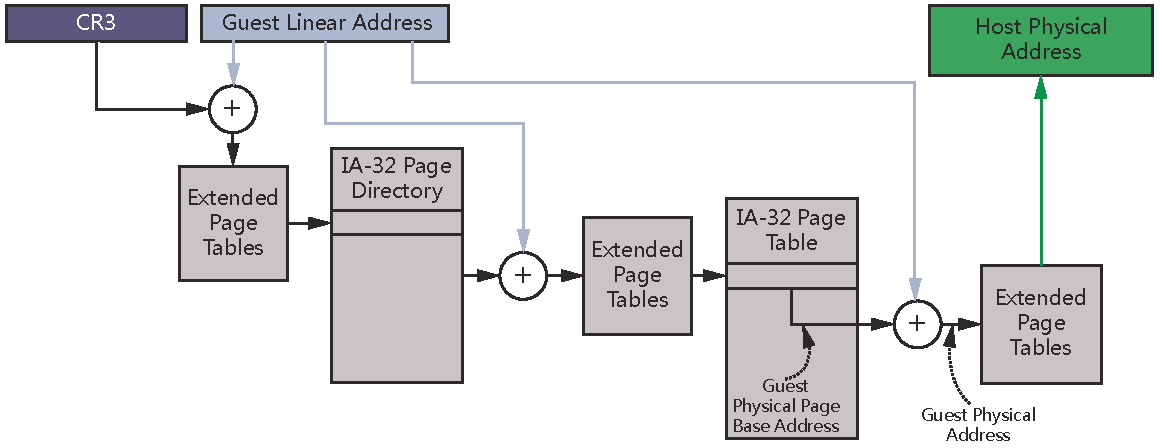
\includegraphics[width=\textwidth]{label/intel-ept-example}
  \caption[Intel Extended Page Table技术示意图]{
    Intel Extended Page Table技术示意图}
  \label{fig:intel-ept-example}
\end{figure}

\textbf{I/O MMU}\quad
IOMMUs are hardware devices that translate
device DMA addresses to proper machine
physical addresses.
which can be used to control how a DMA operation
from a device accesses memory
Intel、AMD和IBM等厂商都提出了自己的I/O MMU方案\cite{intel-iommu, amd-iommu, ibm-iommu},
下文以Intel的I/O MMU为例介绍其功能。

Intel Virtualization Technology for Directed
I/O Architecture provides DMA remapping
hardware that adds support for isolation of device
accesses to memory as well as translation
functionality [2]. The DMA remapping hardware
intercepts device attempts to access system
memory. Then, it uses I/O page tables to
determine whether the access is allowed and
its intended location. The translation structure
is unique to an I/O device function (PCI bus,
device, and function) and is based on a multilevel
page table. Each I/O device is given the
DMA virtual address space same as the physical
address space or a purely virtual address
space defined by software. The DMA remapping
hardware uses a context-entry table that is
indexed by PCI bus, device and function to find
the root of the address translation table. The
hardware may cache context-entries as well as
the effective translations (IOTLB) to minimize
the overhead incurred for fetching them from
memory. DMA remapping faults detected by
the hardware are processed by logging the fault
information and reporting the faults to software
through a fault event (interrupt).



PCI-E标准中使用SR-IOV技术实现I/O设备的共享。

\textbf{Single-Root I/O Virtualization (SR-IOV)}
The Single-Root I/O Virtualization (SR-IOV)
feature is a PCI Special Interest Group (PCISIG)
specification. Intel, along with other
industry leaders, is actively participating in
the PCI-SIG working group to define new
standards for enhancing virtualization capabilities
of I/O devices. SR-IOV provides a
standard mechanism for devices to advertise
their ability to be simultaneously shared
among multiple virtual machines. It also
allows for the partitioning of a PCI function
into many virtual interfaces for the purpose
of sharing the resources of a PCI Express*
(PCIe*) device in a virtual environment. Intel
plans to support the SR-IOV specification in
its networking devices.
Each virtual function can support a unique
and separate data path for I/O-related functions
within the PCIe hierarchy. Use of SRIOV
with a networking device, for example,
allows the bandwidth of a single port (function)
to be partitioned into smaller slices that
may be allocated to specific virtual machines,
or guests, via a standard interface. A common
methodology for configuration and management
is also established to further
enhance the interoperability of various
devices in a PCIe hierarchy. This resource
sharing can increase the total utilization of
any given resource presented on an SR-IOVcapable
PCIe device, potentially reducing the
cost of a virtual system.
Intel-enabled NICs are:
• Intel® 82576 Gigabit Ethernet Controller
• Intel® 82599


\subsection{性能隔离技术}
% CAT/CMT

\subsubsection*{Intel Resource Director Technology(RDT)技术}

针对多处理器芯片中多应用共享的特征,Intel提出了Resource Director Technology方案来解决多应用资源共享冲突问题。
如图\ref{fig:intel-rdt-overview}所示,该方案的硬件基础是资源监控与资源分配控制机制,
同时提供基于``监控->策略->控制''组合的闭环方式来实现应用感知的资源管理框架。
其中资源监控提高了资源使用情况的能见度,使得资源利用率可以被跟踪,同时可以侦测到应用性能随资源的变化,
为上层的资源调度提供数据基础;
而硬件支持的资源分配控制机制,使得上层软件可以控制对硬件共享资源的使用。

% Intel RDT Overview
\begin{figure}[H]
  \centering
  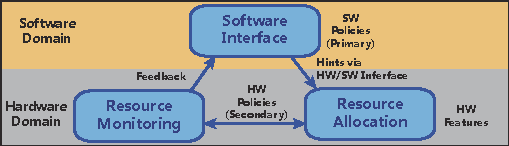
\includegraphics{x86eval/intel-rdt-overview}
  \caption[Intel Resource Director Technology (RDT) 技术示意图]{
    Intel Resource Director Technology (RDT)技术:硬件提供资源监控与分配功能,
    软件负责对资源使用进行调度,实现资源按需求动态分配。}
  \label{fig:intel-rdt-overview}
\end{figure}

目前Intel已经将RDT方案应用到共享末级缓存和内存控制器中,通过CMT/MBM技术实现对缓存容量
以及内存带宽的监控;通过CAT技术实现对缓存容量划分的支持。

CMT和MBM技术允许操作系统或Hypervisor/VMM监控在其上运行的应用对共享缓存与内存带宽
的使用情况,图\ref{fig:intel-cmt-flow}是该技术的流程示意图。
操作系统或VMM首先为执行实体(如线程、进程或虚拟机)分配资源编号RMID,后续的监控结果都将
以RMID的形式进行汇报。在OS/VMM执行调度并进行上下文切换时,将被调度实体的的RMID写入到目标
处理器核对应的寄存器中。OS/VMM可以随时通过RMID查询各个执行实体的资源使用情况,如共享缓存
占用或访存带宽等信息。
 
% Intel CMT Flow
\begin{figure}[H]
  \centering
  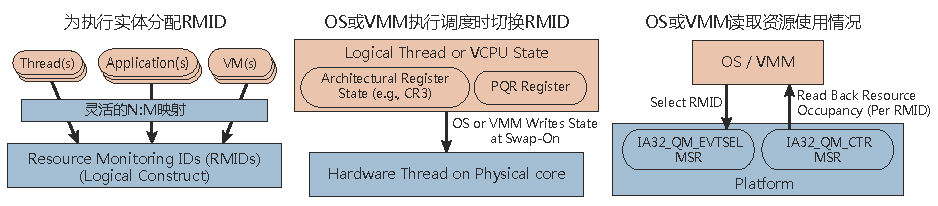
\includegraphics{x86eval/intel-cmt-flow}
  \caption[Intel Cache Monitor Technology (CMT) 技术流程]{Intel CMT技术流程:
   (1)为线程、应用或虚拟机等执行实体分配资源编号RMID;(2)将包含RMID的PQR寄存器
   保存在线程TCB或虚拟机VCPU中,并在执行上下文切换时写入到处理器核对应的物理寄存器中;
   (3)根据RMID使用MSRs寄存器获取共享资源使用情况。}
%Threads, applications, VMs or any combination can be associated with an RMID, enabling very flexible monitoring. As an example, all threads in a VM could be given the same RMID for simple per-VM monitoring. (2) The PQR register (containing an RMID) stored as part of a thread or VCPU state, which is written onto the thread-specific registers when a software thread is scheduled on a hardware thread for execution. (3) After a period of time (as defined by the software) the occupancy data for a given RMID can be read back through a pair of keyhole MSRs which provide the ability to input an RMID and Event ID (EvtID) in a selection MSR, and the hardware retrieves and returns the occupancy in the data MSR.}
  \label{fig:intel-cmt-flow}
\end{figure}

CAT技术为OS/VMM提供了控制末级共享缓存容量的功能,如图\ref{fig:intel-cat-flow}所示,
当该功能被开启后,应用将只能使用分配给它的Cache容量,实现路划分。
路划分策略是以COS为粒度进行指定,OS/VMM首先为某一COS制定路划分策略,并将该COS关联到使用
该策略的执行实体中,并在上下文划分时将被调度实体的COS写入到处理器核对应的寄存器中,
共享缓存根据COS对应的策略来进行缓存替换操作。

\begin{figure}[H]
  \centering
  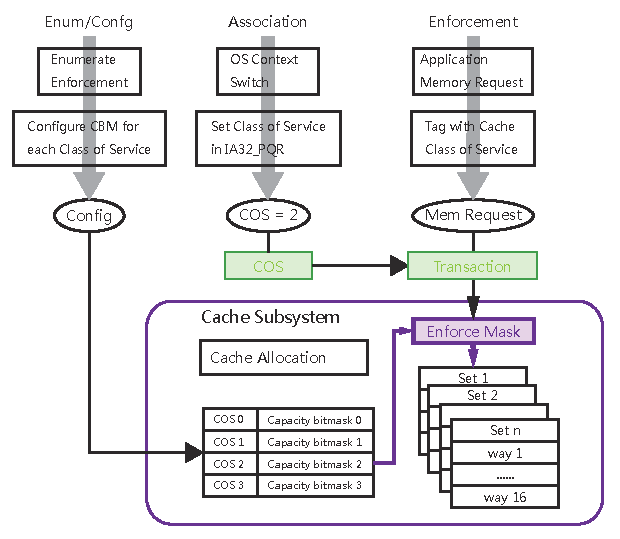
\includegraphics[height=8cm]{x86eval/intel-cat-flow}
  \caption[Intel Cache Allocation Technology (CAT) 技术流程]{Intel CAT技术流程}
  \label{fig:intel-cat-flow}
\end{figure}



\section{标签机制}

在之前的章节中已经对PARD的标签机制进行了介绍,简单来说其核心包括两点:
一是如何为计算机中的请求\textbf{标记}上正确的标签,
二是保证标签在整个计算机系统中正确\textbf{传播}。
但在具体实现标签机制时,仍然有一些问题需要考虑,
本节主要讨论其中的标记问题,传播问题将在下一节中讨论。


\subsection{标签粒度与格式}

PARD对用户提供了逻辑域抽象,因此简单的标签方案可以直接将一个逻辑域映射到为一个标签,
以逻辑域为粒度分配系统内的硬件资源(资源划分),
并对共享硬件资源的访问进行控制(性能划分),
本文所设计的FPGA原型系统(参见第\ref{chap:impl}章)选择了该方案进行实现。
另一些应用,需要在逻辑内也实现性能划分,
即运行在同一个逻辑域的不同应用具有不同的资源访问级别,
基于容器的技术的轻量级虚拟化即属于该类型,运行在不同容器中的应用虽然具有不同的优先级,
但它们能够访问相同的资源。
为了支持这种类型的应用,本文提出了两级标签的概念,如图\ref{fig:tagging-format}所示,
将标签划分为资源域与性能域两部分,
不同资源域的应用在硬件资源上相互隔离,且具有不同的性能策略;
具有相同资源域的应用共享同一份硬件资源,
但这些共享的硬件资源使用不同的性能策略来处理来自不同性能域的应用。

\begin{figure}[tb]
  \centering
  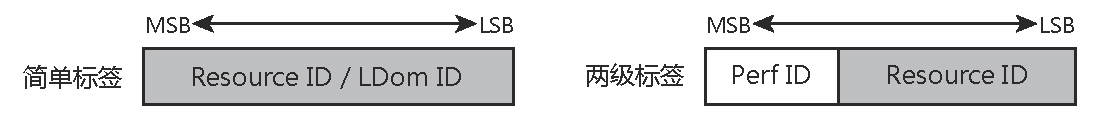
\includegraphics[width=\textwidth]{label/tagging-format}
  \caption[标签格式]{标签格式:分为简单标签与两级标签,
    简单标签直接将逻辑域(LDom ID)映射为标签,
    两级标签将标签分为资源域(Resource ID)和性能域(Perf ID)两部分。
    只有两级标签的性能域部分可以由用户进行修改,
    简单标签或两级标签的资源域(图中阴影部分)只能通过PRM进行修改,
    以保证硬件资源分配不会出现冲突。}
  \label{fig:tagging-format}
\end{figure}

\subsection{如何为请求打标签}
\label{chap:labeladdrspace:tagging}
在确定了标签的格式与内容后,需要将该标签打到对应的请求上。
在计算机中存在两个请求发起源,即处理器核与I/O设备的DMA引擎,
需要在这两个请求源将应用标签标记到请求上。
% 外部标签也在该节讨论

\begin{figure}[b]
\begin{minipage}{0.48\textwidth}
  \centering
  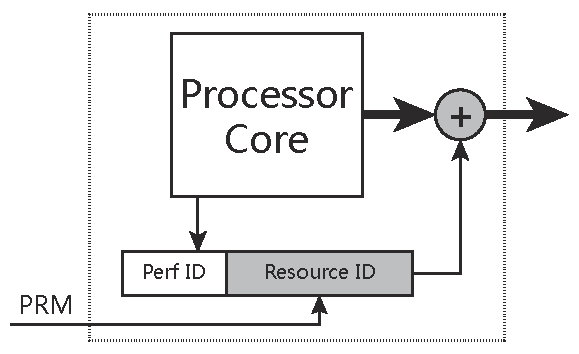
\includegraphics[width=0.9\textwidth]{label/tagging-core-request}
  \caption{为处理器核请求打标签}
  \label{fig:tagging-core-request}
\end{minipage}\hfill
\begin{minipage}{0.48\textwidth}
  \centering
  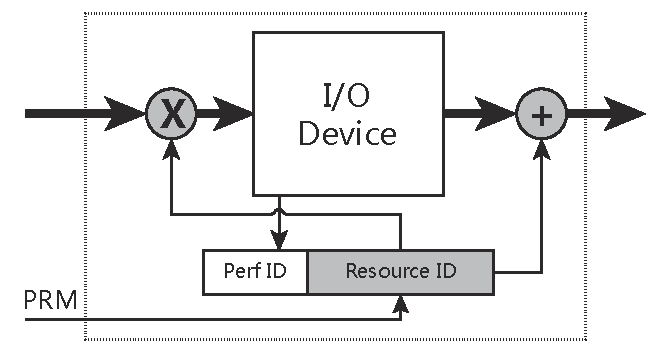
\includegraphics[width=0.9\textwidth]{label/tagging-io-request}
  \caption{为I/O请求打标签}
  \label{fig:tagging-io-request}
\end{minipage}
\end{figure}

\textbf{处理器核}\quad
为实现处理器核发出的请求的标记,
需要在处理器核内增加一个标签寄存器,将当前正在使用该处理器核的应用标签保存在该寄存器中。
对于简单标签模式,该寄存器对处理器核不可见,只能通过PRM在逻辑域切换时进行修改;
对于两级标签模式,该寄存器的性能域部分对处理器可见,
可以由逻辑域内的操作系统在进行切换时进行修改,而资源域与简单模式下相同,只能由PRM进行修改。
图\ref{fig:tagging-core-request}给出了两级标签模式下,处理器核的请求标记过程:
处理器核发出的请求与标签寄存器的值进行组成,形成带有标签的请求发送到外部;
标签寄存器的资源域部分只能由PRM进行修改,性能域部分可以通过处理器核进行修改。
%处理器核共享场景(0.1个处理器核)也许需要具体一下

\textbf{I/O与中断请求}\quad
对于I/O访问,有两种访问模式,即Programmed-I/O(PIO)和Directed Memory Access(DMA)。
对于PIO访问请求,由于I/O请求已经在处理器核端进行了标记,
因此在设备端直接将请求所附带的标签返回即可,但对于DMA请求进行标签标记则需要进行额外的处理。

在介绍PARD的DMA请求标签机制前,先对DMA的工作原理进行简要回顾。
通常一个DMA请求过程可以分为三个阶段:
首先设备驱动发送一个``DMA描述符''首地址到DMA控制器,
该``DMA描述符''包含了DMA的缓存信息,例如起始地址、缓存大小、状态;
当初始化完成之后,DMA控制器加载描述符,从中获取每个DMA操作必要的信息并开始数据传输;
最后当所有数据都传输完成后,DMA控制器产生中断告诉CPU数据处理完成。

为了实现DMA请求的标签机制,PARD在每个DMA控制器中都加入一个``标签寄存器'',
如图\ref{fig:tagging-io-request}所示。
在逻辑域创建过程中,PRM对设备进行分配,将逻辑域的资源标签写入到该标签寄存器中。
对于DMA请求的三个步骤,标签寄存器相应的操作如下:
(1)初始化标签寄存器性能域并读取DMA描述符。当设备驱动向DMA引擎写如DMA描述符信息的同时,
将请求相关的标签性能域部分写入到标签寄存器中,
DMA引擎将标签寄存器中的值附加到DMA描述符读取请求中。
(2)标记数据传输请求。当设备的DMA引擎与内存控制器进行收发数据时,
从其标签寄存器中取出标签,将每个数据传输请求上都打该标签。
(3)标记中断信号。对于中断,PARD对当前的中断控制器
(Advanced Programmable Interrupt Controller, APIC)进行适当的扩充。
在APIC中增加多个中断映射表,其中的每一个都与一个应用标签进行关联。
这样当DMA引擎将要产生一个中断时,把应用标签标记到中断请求中,然后发往APIC。
APIC使用请求中的应用标签来获取相关的映射表,
根据表中的信息将中断请求转发给指定的处理器核。



\section{标签传播}
\label{chap:labeladdrspace:propagation}

标签需要伴随请求在整个生命周期中传播,
这些不同类型的请求需要在各种协议类型的总线上传播(如QPI/HT、AXI、PCI-E等),
其间需要进行多次协议转换,同时会多次穿过各种Cache与Buffer,
本节首先讨论如何扩展现有的总线架构,使其能够传递标签信息,并讨论如何在保证在传播过程中请求与标签始终匹配。
%计算机中的请求主要分为三类:处理器发出的读写请求、I/O设备发出的DMA请求、中断请求。

\subsection{总线与协议转换}

不同总线上如何实现地址空间


\subsection{一致性协议}

% 侦听和目录两种协议,目前大都使用目录(扩展性原因)
% Source-Snooping 1-2 sockets    <= need reference
% Home-Snooping   4+ sockets
% Directory       64+
PARD使用共享内存多处理器架构,每个处理器都包含自己的私有缓存,
需要使用一致性协议来保证这些私有缓存的一致性。
最常用的保持一致性的方法是基于侦听或基于目录,它们各有优缺点,
基于侦听的方法的优势是响应速度快,所有的请求通过一次广播的请求和回应即可完成,
但它带来的问题是链路带宽占用过大,尤其是当核数增加时,其带宽占用也越来越大。
基于目录的方法主要解决带宽占用问题,通过使用一个公共的目录来记录所有数据的缓存情况,
在需要执行无效操作时,只将请求发送到包含该数据的节点,可以使用点对点的连接,
而无需广播,降低的带宽占用,但与此同时也增加了响应延迟
(需要request/forward/respond三跳)。
Intel的实验\cite{}表明在四核以下使用基于侦听的方法,
而更多的核数后需要使用基于目录的方法以降低开销。

% PARD需要对目录项进行修改,以保证正确性
当前处理器核数不断增加,目前普遍的服务器都具有24个处理器核,
这些服务器大都采用基于目录的一致性。
图\ref{}是基于目录的一致性协议的执行流程,首先....。
由于PARD使用标签的方式区分不同逻辑域的地址空间,因此系统中存在多个重叠的地址空间,
需要使用标签来区分这些地址空间,
因此,PARD修改了目录项的定义,将标签信息也加入到目录项中,
在进行地址对比时需要同时对比地址与标签,只有两都同时匹配时才将语法转发到该结点。

% 云计算场景下,每个虚拟机核数较少,可以使用局部侦听的方法实现快速的一致性,
% 同时开销也可控
再次考察基于侦听的一致协议,其在少数节点时性能要高于目录一致性协议,
主要是由于当前服务器中核数增加,链路带宽不足,因此才被抛弃,
转而使用实现更为复杂的目录一致性协议。
当前多租户云计算场景下,虽然服务器本身具有大量的处理器核(>24),
但每个用户的虚拟机通常只使用的处理器核\cite{},    % <= need reference
由于虚拟机之间无内存共享,因此可以只在所有处理器的一个子集中实现一致性,
在这样的范围下,使用基于侦听的一致性可以提高性能,同时由于节点数据较少,
广播开销也不大;特别的,当只使用一个处理器核时,可以忽略所有一致性相关的请求,
进一步降低一致性开销。

PARD的标签化地址空间为以上的一致性协议提供了支持,
即只需要将一致性请求发送到与其标签相同的处理器核,
而无需在全局范围内广播或进行目录查询操作。

% 即使虚拟机的核数较多,也可以使用局部目录一致性,降低目录存储开销

% 结论,标签化地址空间以及逻辑域抽象,可以实现局部一致性协议,
% 通用逻辑域核数决定一致性协议的类型(甚至是不需要一致性,单核)

\subsection{多内存控制器}

随着处理器核数不断增长,单个内存控制器性能无法满足处理器核的需求,
现有体系结构实现通常包括多个内存控制器\cite{},
处理器需要提供一种机制实现物理地址空间在多个内存控制器的分布,
并为请求提供地址解码支持。
以Intel的Xeon架构为例,其使用Source Address Decoder(SAD)
和Target Address Decoder(TAD)实现地址空间管理\cite{intel-xeon-7500}。
其中SAD位于Cache Box(Cbox),负责将请求地址解析到对应的I/O或内存控制器
(对于interleave的地址,则是一组控制器),本节主要讨论对内存地址的解码;
而TAD位于Home Agent(Bbox),负责将请求地址解析为本地地址(主要是处理interleave情况),
并将解析后的地址发送给内存控制器(Mbox)完成访存请求。

SAD的结构如图\ref{fig:intel-7500-sad}所示,\textbf{把这个图改造成PARD的结构,增加PRM和DSid索引的表,}
其中包含一个20项的译码表,输入为请求地址,
输出为路由目的地列表,并交给Router模块转发请求。
在Intel的这种体系结构下,请求路由是由请求地址决定。
在PARD体系结构下,需要综合考虑请求地址与应用标签,
PARD对译码表进行扩充,在系统中预留多组译码表(组数由支持的最大逻辑域数量决定),
这些译码表按逻辑域标签索引,当PRM决定在某个处理器核上运行一个逻辑域时,
需要将该逻辑域对应的译码表加载到处理器中,
这样保证该处理器核在做地址译码时使用对应用逻辑域的地址分配。

\begin{figure}[tb]
  \centering
  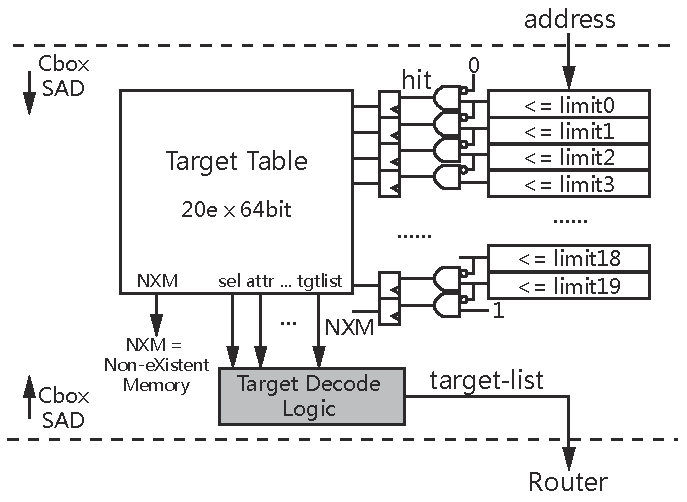
\includegraphics[width=0.7\textwidth]{label/intel-7500-sad}
  \caption[Intel SAD地址译码]{Intel SAD地址译码}
  \label{fig:intel-7500-sad}
\end{figure}


\subsection{多阶段写回请求}

为了提高性能,计算机数据通路中采用写回(writeback)机制的写操作通常会被拆分成多个阶段。
以共享末级缓存为例,写请求的第一阶段只是将数据写入到缓存中,并将其所属的数据块标记为脏块,
只有当缓存缺失发生且该数据块被选择为替换备选时,数据才会被真正写回到内存。
如果仅使用末级缓存所接收到请求的应用标签作为写回请求的标签,可能会产生标签错误:
引起写回操作数据所属的应用与被写回的数据所属的应用不一致。
为了防止这种情况的发生,需要在共享末级缓存中,
为所有缓存的数据块额外记录其所属应用的标签Owner-DSid,
在第一阶段数据被写入缓存时,将写请求中包含的DSid记录为其Owner-DSid;
当写回操作发生时,使用其Owner-DSid作为传递到下一级的标签。
其它与共享末级缓存行为类似的具有写回机制的部件,都需要应用以上的改,
才能保证请求在通过该部件后保证应用标签的正确性。

\subsection{中断}


\section{标签应用:实现全硬件虚拟化NoHype}

通过利用本章所设计的标签化地址空间架构,通过应用标签以及相应的标签传播机制,
实现在整个计算机体系结构内识别出来自不同应用的请求,
本节将讨论如何利用该架构实现全硬件支持的虚拟化技术,实现PARD的逻辑域抽象。

要实现无Hypervisor辅助的全硬件虚拟化,首先回顾一下Hypervisor在整个虚拟机生命周期中的作用,
然后讨论如何在标签化地址空间的架构下,使用硬件逻辑来替代Hypervisor的工作。


本文基于gem5\cite{gem5}模拟器,在X86指令集的TimingSimple访存模型下实现了标签化地址空间,
本节将对该模拟器的实现进行简要分析,并讨论如何通过标签化地址空间实现无Hypervisor的全硬件支持的虚拟化。

在第\ref{chap:labeladdrspace:related}节中介绍了现有技术中如何实现资源共享与性能隔离,
本节将使用标签化地址空间实现这些功能,包括:地址空间隔离、I/O设备共享、
以及Cache容量划分。

\subsection{地址空间隔离}

在现有技术中使用EPT与I/O MMU技术实现地址空间隔离,
其中EPT用于实现处理器端请求地址的隔离,I/O MMU用实现DMA设备端的地址空间隔离。


地址映射位置,与EPT+I/O MMU技术对比

Cache一致性场景下如何实现标签化地址空间


\subsection{I/O地址空间隔离}

SR-IOV or pseudoMR-IOV
I/o protect bitmap

\subsection{通过标签实现Cache容量划分} %性能隔离

本文所提出的标签化地址空间机制,使用统一的标签实现资源隔离与性能隔离。


\subsection{PARD标签化地址空间模拟器实现}



\begin{figure}[tb]
  \centering
  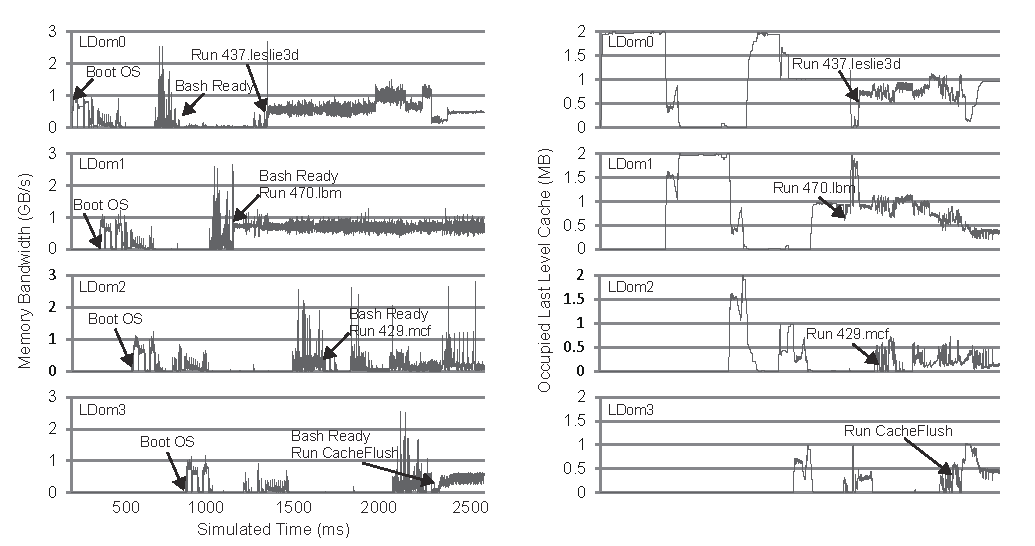
\includegraphics[width=\textwidth]{label/pard-nohype-simulator}
  \caption{动态划分一个PARD服务器为四个逻辑域,并在其中运行操作系统与应用}
  \label{fig:pard-nohype-simulator}
\end{figure}

\section{小结}


\if 0

\section{体系结构的可行性}

在X86或ARM上实现该架构

%如何在一个ARM中实现PARD功能

如上节所述,PARD并不是一个完全全新的体系结构,而是对现有体系结构的扩展。
为了说明如何将PARD扩展到一个现有的体系结构中,本节首先构建了一台虚拟计算机,
我们将其命名为XXXX,如图\ref{fig:XXX-computer}所示。
XXX包含两路4核的处理器,每个处理器核拥有独立的一级缓存L1-I和L1-D,
每个Socket的四个处理器核共享一个16路2MB的二级缓存;
两个Socket拥有自己的内存控制器,同时使用MESI目录协议实现NUMA内存访问;
XXX的I/O子系统包含SATA控制器和两个以太网卡,通过IOH芯片与两个处理器相连。
XXX的结构可以很好的匹配到目前流行体系结构中(如X86或ARM)。

\subsection{Computer as a Network => PARD}

\subsection{像SDN一样集中式的管理计算机}

\section{PARD与SDN}

在第\ref{chap:intro}章中我们提出
同时,计算机内部也可以被看做一个网络,如图\ref{fig:computer-as-a-network}所示,
CPU核、共享缓存、内存控制器、I/O设备等可以被看做是网络节点;除了处理请求以外,
这些``网络节点''与网络中的路由器/交换机具有相似的请求转发功能;
而它们之间也通过包进行通信,如:片内通信使用NoC包,片间通信的QPI/HT包,
以及I/O部分使用的PCI-E包。
将网络领域的区分化服务和软件定义网络的思想应用到计算机内部的网络,
用以解决数据中心当前面临的资源利用率与应用服务质量矛盾,是本文的主要研究思路与动机。

与在网络中部署SDN相比,在计算机体系结构``网络''中部署SDN会面临以下三个挑战:

首先,在整个网络栈中EndPoint是唯一的请求来源,因此SDN可以很容易的将标签机制实现在网络栈中;
与之相对的,在计算机体系结构中存在大量的硬件部件都能够发送请求,而这些请求类型又不尽相同,
因此在这样的环境下如何为请求打上标签是一个很大的挑战。

其次,在网络中所有的交换机都执行相同的存储/转发(store-and-forward)操作,但在计算机内部
不同的部件都有不同的功能,而不只是简单的存储/转发,如何为这些不同类型的部件(如末级缓存控制器、
内存控制器、I/O设备等)设计统一的控制面结构是另一个挑战。

最后,在网络交换机中已经包含了一个firmware固件用于访问和配置交换机的控制面,但计算机中却缺少
这样的firmware。现有的IPMI只被用来做有限的监控与管理功能,如对温度、风扇转速和电源控制。
因此,需要在计算机内部提供一种这样的部件实现与其它众多的控制面的通信与管理,并提供一个灵活的
编程接口对这些控制面进行操作。

\fi
